\documentclass[conference]{IEEEtran}
\usepackage[pdftex]{graphicx}
\graphicspath{{images/}}
\usepackage[backend=biber, style=ieee]{biblatex}
\addbibresource{jprefwolf.bib}
\addbibresource{mwrefwolf.bib}
\usepackage{amsmath} % For better math in tables and equations
\usepackage[final]{microtype} % Makes things look better in the end
\usepackage[hidelinks]{hyperref}
\usepackage{listings}

% correct bad hyphenation here
%\hyphenation{op-tical net-works semi-conduc-tor}

\begin{document}
%
% paper title
% Titles are generally capitalized except for words such as a, an, and, as,
% at, but, by, for, in, nor, of, on, or, the, to and up, which are usually
% not capitalized unless they are the first or last word of the title.
% Linebreaks \\ can be used within to get better formatting as desired.
% Do not put math or special symbols in the title.
\title{The Wolf in Sheep's Clothing:\\
Subversive Adversarial Agent Identification}


% author names and affiliations
% use a multiple column layout for up to three different
% affiliations
\author{\IEEEauthorblockN{Jean P. Castillo\IEEEauthorrefmark{1},
Matthew W. Swartwout\IEEEauthorrefmark{2}, Russell C. Jackson\IEEEauthorrefmark{3} and
Murat C. Cavusoglu\IEEEauthorrefmark{4}}
\IEEEauthorblockA{Department of Electrical Engineering and Computer Science,
Case Western Resere University\\
Cleveland, OH 44106\\
Email: \IEEEauthorrefmark{1}jpc87@case.edu,
\IEEEauthorrefmark{2}mws85@case.edu,
\IEEEauthorrefmark{3}rcj33@case.edu,
\IEEEauthorrefmark{4}mcc14@case.edu}}

% conference papers do not typically use \thanks and this command
% is locked out in conference mode. If really needed, such as for
% the acknowledgment of grants, issue a \IEEEoverridecommandlockouts
% after \documentclass

% use for special paper notices
%\IEEEspecialpapernotice{(Invited Paper)}

% make the title area
\maketitle

% As a general rule, do not put math, special symbols or citations
% in the abstract
\begin{abstract}

Mobile robot security is a rapidly developing area of interest in robotics. As interconnected mobile robotic systems become more ubiquitous, the need for security and reliability continues to grow. One avenue for advancement in this is distributed systems coordinated between multiple agents. This paper proposes a state detection system validation which allows agents to detect compromised agents in their environment. Security is retained by means of a distributed state estimation system that uses Kalman filters and a secure ad-hoc channel to manage communications between the agents. The detection of such compromised agents can be used to create a \textit{trusted set} within a group, providing a multi-node trust system. A TurtleBot running Robot Operating System (ROS) platform is used for implementation and performance is also evaluated in the Gazebo simulator.

\end{abstract}

% no keywords


% For peer review papers, you can put extra information on the cover
% page as needed:
% \ifCLASSOPTIONpeerreview
% \begin{center} \bfseries EDICS Category: 3-BBND \end{center}
% \fi
%
% For peerreview papers, this IEEEtran command inserts a page break and
% creates the second title. It will be ignored for other modes.
\IEEEpeerreviewmaketitle

\section{Introduction}
Robot security has landed headlines across a variety of commonly used networked devices, car hacking being a prominent example of a security flaw that could have catastrophic impact in the United States and abroad. Some individuals have been able to remotely connect to, disable, and control various vehicles in the market through techniques like that of \textcite{greenberg2015hackers}, posing many questions about the protocol used in vehicles and how other cars in the same network can work to detect and isolate a compromised agent. This network of agents come in a combination of centralized and distributed characteristics in order to achieve a common goal. Centralized systems have the advantage of control and lower cost at the expense of one central point of failure, whereas a well structured decentralized system can be resilient to various attacks due to its versatility. As more agents become connected, much like cyber-vehicles in a highway would, decisions that each agent makes can be based on the information it obtains from not only its sensors but also other agent's data. This paper discusses how an agent can securely obtain the probability that another agent in the system is compromised in order to trust feedback obtained from that agent in question.

There are three core goals for the security of any cyber-physical system: integrity, availability, and confidentiality \cite{Cardenas2008}. Those can be thought of as three simple questions: ``Can I trust the data?'', ``Do I have access to the data when I need it?'', and ``Is the data hidden from those who shouldn't have it?''. In a trust chain there is an initial block of trust called Hardware Security Engine (HSE) unit which fingerprints specific physical properties of the hardware to uniquely identify an agent. This fingerprint is used to verify various modules of an agent such as the static software, dynamic software, control system and communication between agents.

Communication between two agents focuses on confidentiality and integrity which can both be accounted for through proper encryption and meta-data inside the encrypted message. A challenge-response system is implemented in this paper which changes on every round trip time providing fresh keys for the uniquely encrypted payload. Timestamp and source mac address fields inside the encrypted payload not only ensure the identity of the sender, but also the timing integrity. Once communication is secured, an adversary can still distort the sensor data of an agent however. An agent in the group can detect the abnormality by comparing the state and behavior combination taken to that of an established \textit{usage envelope}, a pre-computed state trajectory map. This map allows for a large variety of planning algorithms to be used. The state of the agent is computed through the use of redundant measurements in the system which allow for an agents inside a trusted set to verify each other's locations.

The remainder of the paper will continue as follows. Related work pertaining to integrity, availability, and confidentiality will be presented in \ref{sec:Related Work}. The system design is introduced in section \ref{sec:Methodology} which further discusses the implementation techniques used. We then demonstrate our experiments in section \ref{Results} and the results obtained in section \ref{Results} and gather a conclusion from the results and motivation of the paper in section \ref{Conclusion}.

\section{Related Work} \label{sec:Related Work}
Chain of trusts of agents have been introduced in works such as that of~\textcite{adi2009mechatronic} where a DNA ideology was utilized to formulate a clone resistant agent; a Physical Unclonable Function (PUF) was introduced which obtains physical differences between other electronic devices. Similar to this work the extended chain of trust this paper is the HSE which is used to verify other parts of the system much like~\textcite{adi2009mechatronic}. We focus the distributed system aspect and begin through a look into what it means to verity the behavior of another agent.

\subsection{State Estimation}
State estimation is a fundamental problem for robotics. Without knowing its location, a robot cannot be very useful. One common technique for robot localization is to use a Kalman Filter (KF). The KF is one of the most studied and most heavily utilized Bayesian filter~\cite[39-81]{ProbabilisticRobotics}. The application of the KF to the task of robot localization has been studied intently~\cite{Localization2003, Mohsin2014} and can hence be used as an external measure of identification for a robot's behavior. For this paper, we utilize an Unscented Kalman Filter (UKF) for the task of sensor fusion and localization as it provides superior results to that of the EKF \cite{Thrun2002Probabilistic}.

\subsection{Secure State Estimation for Distributed systems}
Secure State Estimation in a distributed system requires a focus on all three of the previously mentioned facets of security: Integrity, Availability and Confidentiality. We choose to focus on the first and third of these, Integrity and Confidentiality, for our secure estimation system.

\subsubsection{Integrity}
Integrity is the question of whether or not the state estimation system's output is accurate. We propose two primary failure modes for integrity: sensor failure and false data injection.

In a total sensor failure scenario one or more of the sensors will stop providing all feedback. This is something that KFs can handle without problem. The KF is always using all available information to generate its state estimate, and if one sensor fails the only result is that the accuracy of the filter will decrease. If 100\% of sensors fail, the filter will become non-functional, but this would affect any state estimation system. The KF also does not have issues with sensors going in and out of a failure state. When information is available it is used, and when it is not available the sensor can be ignored.

Sensor failure is not a huge risk for the KF, but  sensor interference is a much more complex problem. If an attacker is able to inject false data, the localization estimate can be skewed. This is a very real problem with many ways that false data could be added, ranging from physically blocking a LIDAR sensor to hijacking the network packets of a wireless sensor.

\textcite{Mo2010, Yang2013} demonstrate that KFs are susceptible to false data injection attacks, and that even with failure detectors, a clever adversary can craft their attack to bypass these detectors. \textcite{Bezzo_2014, Mo2014} attack this problem by adding extra steps to their KF algorithm. Both successfully show that the filter output can be shielded from the effects of the false data injection attack.

\subsubsection{Confidentiality: Secure Ad-Hoc Channel Communication}
There are various works that cover a communications for adhoc networks. ~\textcite{vegh2014securing} uses an extension of the ElGamal algorithm in order to limit the access of agents in the network. In the event that an agent is compromised the information within the decrypted message remains protected through steganography, a method used for hiding information within a text \cite{adi2009mechatronic}. The implementation uses direct agent to agent communication and thus no hierarchy is used; no encrypted broadcast messages are sent and it seems unnecessary to encrypt the information further as it would lead to potential DOS attacks.

Another protocol introduced in ~\textcite{chang2016provably} provides forward secrecy through registration, authentication and password changing involving communication between user, sensor and gateway nodes. A long term secret is used for the session and a change in password occurs once the connection is established; however, in a moving environment there may instances when only two nodes will be able to communicate at one time.

In the field of automobiles~\textcite{lyu2016pba} developed a protocol named PBA that is well guarded against high traffic and lossy wireless networks.~\textcite{lyu2016pba} also addresses Denial of Service (DOS) attack resistance and stores shortened keys for less memory consumption and rapid verification~\cite{lyu2016pba}. ~\textcite{lyu2016pba} takes a private public key pair approach which may be prone to further attacks as the base station could update their keys~\cite{lyu2016pba}. Connectivity to the central station after the release is not taken to be necessary in this paper's approach, yet obtaining accurate clock synchronization for distributed systems such as that surfaced in ~\textcite{Park2016method} is helpful to guard against attacks.

\subsection{Distributed State Estimation}
As single robot systems coalesce into functional teams, distributed state estimation systems are desirable. Traditionally, in order to increase the accuracy of state estimation, more sensors are added to an individual robot. These additional sensors increase the cost and complexity of the robot. An alternative solution is for robots to share their sensor readings with others in their environment. This increases the amount of sensor data available to each robot, while keeping the number of sensors low on any one robot.

Most research into such systems relies on the concept of cooperative positioning~\cite{Kurazume1994} where robots coordinate their motions so that they can localize, or aid in the localization of, other robots. Often this involves one robot acting as a stationary landmark while the other robot moves. Studies done on this system have shown its effectiveness~\cite{Kurazume1996, Kurazume1998, Kurazume2000}. This is a valuable concept when working with a team of coordinated robots. However, many systems will not allow for cooperation.

Other work still makes the assumption of a cooperative team, even when they don't rely on cooperative positioning. \textcite{Sanderson1997, Roumeliotis2002} both demonstrate a system where a KF is implemented that estimates the state of multiple robots in a system. However these states are computed relative to each other, representing the network of robots as one large robot with different parts.

The previously mentioned works are all examples of a decentralized, rather than distributed KF problem. \textcite{Olfati-Saber2005} makes clear the distinction between these two, explaining that a decentralized method requires a complete connection between all nodes in the system, whereas a distributed system does not.

One truly distributed solution uses consensus filters and multiple KFs~\cite{Olfati-Saber2005}. However this still requires adaptation of the KFs and extra computation, which is something we try to avoid. In this paper we will show a distributed system with minimal KF modifications, and not a decentralized one. 

\subsection{State Detection}

In order to obtain a road-map of appropriate behaviors an compromised agent can exhibit in a given environment, different types of planning have been introduced in literature. Complex environments can be made up of many possible paths which can be computed with strategies such as that of ~\textcite{tallavajhula2016list}, where each iteration of path planning uses a more complex predictor. Each of these predictors' path can be used to build a map of states and corresponding behavior that an agent is able to perform. Other planning algorithms use specialized planning based on a sub process task such as ~\textcite{ahn2008robust}'s vertical control system, where one module is independently responsible to avoiding objects while more abstract modules can plan according to behavior of objects.

\subsection{Work Contribution}
Mapping a robot's trajectory can be done by trivial means, mapping those behaviors to predefined paths can also be seen in <>. The novelty of the work in this paper comes from the view point of utilizing mapped behaviors in order to make predictions on whether the robot is compromised from a robotics perspective whereby security must be considered. Through an agent's detected state we are able to demonstrate a building block for trust within a secured distributed system of robots, one which may be used as a measure to detect whether or not an agent is likely to be compromised by means of sensor failure or false data injection.


\section{System Design} \label{sec:Methodology}

The method in which the three strategies of interest are implemented are now outlined. The reader should make note the intended chain of trust commences with hardware integrity at its core moving through the various levels of authentication for integrity self-verification.

\subsection{Secure Ad-Hoc Channel Communication}

The communication between agents must be encrypted with secret and unique keys. In addition future releases of a robot must be able to communicate with the existing versions. A HSE can be used in order to provide security as seen in \autoref{conn_alg}.

\begin{lstlisting}[language=Python, frame=single, columns=flexible, label=conn_alg,caption={Algorithm used to compose encrypted payload}]
def prep_send_packet(skt, dest_mac, payload):
	CR = get_host_CR(dest_mac)
	enc_msg = construct_msg(payload,CR[0], CR[1])
	send_packet(skt, dest_mac, enc_msg)
	
def get_host_CR(mac):
	dest_mac_enc	= HSE.compute_hmac(mac)
	return HSE.dec_CR(db_enc[dest_mac_enc])
	
def construct_message(payload, challenge, response):
	pickle_array = dumps(payload,2)
	eth_header = HSE.MAC + get_timestamp() 
	                        + HSE.new_CR()
	msg = eth_header + pickle_array
	return challenge + HSE.enc_msg(response, msg)
\end{lstlisting}

A cryptographically random challenge is produced for which there is a globally known one way function to compute a response by means of the originating party's hardware signature, this response is what will be used as input to the encryption/decryption cypher of choice. Naturally the receiver will not have the hardware signature of the originator, and thus we must use a unique table entry for each agent in the system that is created upon initializing the agent itself, mapping each MAC address, or agent identity, with a Challenge Response (CR) pair obtained from the trusted source. These keys are very important and therefore, in order to comply with privacy we must be able to change keys as to avoid decryption attempts. For this the use of churn will be utilized whereby a new CR pair to be used will be sent with every packet exchanged; that is, the sender sends a new cryptographically generated random C-R pair that the each agent's table may be updated with for the next packet to be sent. In order for the receiving party to know the message decrypted is in fact legitimate there must be text that can be verified. There is also need to verify who the message came from due to our authenticity requirement as the packet's Ethernet frame can easily be replayed by a man in the middle. These can both be satisfied by placing the source MAC address in the encrypted portion of the message exchange. 

To further protection we place the MAC of an agent inside the HSE to make it part of its immutable identity. Replay attacks can also be a danger, and the method of guarding is having an accurate timestamps.
	
New agent authentication work in a similar manner to normal communication but must be initiated by the party with the appropriate and working CR pair. Last but not least, this communication must be implemented like a tunnel where each agent can be uniquely identified by the system.

\subsection{State Detection}

We start our state detection by defining our local frame state and control as $\dot{x}$ and $\dot{c}$ respectively. The following outlines how the process of obtaining the probability of being compromised from the sensory inputs and the desired method of path planning.

Now that we have a defined state we must gather the state from a combination of sensor data and information obtained from the robot. We use a particle filter for this purpose which we initialize to cover the full area of interest. If an initial position is provided a particle is given that claimed position, but all others are kept in their random position to accommodate for a false given position.
	
We obtain the average of the particles  which is utilized in order to obtain an approximate point nearest to some neighbors on two maps: a compromised map and an uncompromised map. Both maps are comprised of state points along the path planned that are considered compromised or uncompromised as illustrated in figure~\ref{fig:compmaps}.
	
\begin{figure}[]
\centering
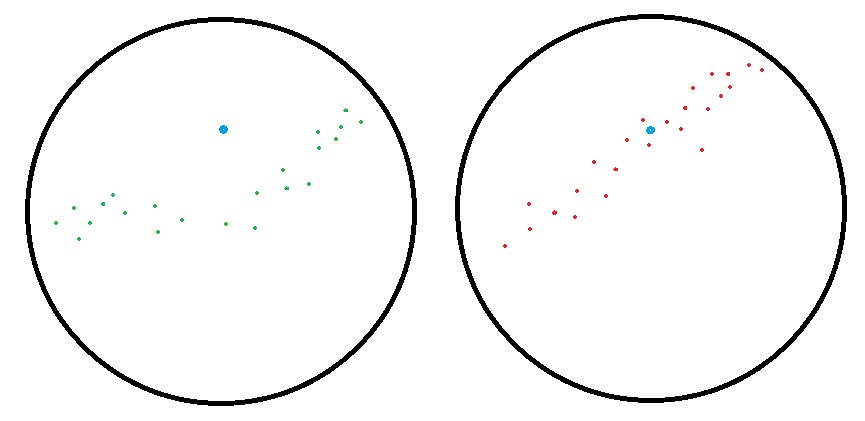
\includegraphics[width=0.4\textwidth]{Path_comp_uncomp}
\caption{The left shows the uncompromised map made up of states avoiding some area and the right shows a compromised map where the states do cross the same area. In this case the state obtained from the particle filter mean, demonstrated in blue, would likely yield a more compromised probability}
\label{fig:compmaps}
\end{figure}
	
A KD tree is used on both maps to find the closest approximate points to each mean found. The few particles gathered by this process are used, by the compromised and uncompromised maps, to form probability density function (PDF) by means of a Kernel density estimation (KDE). This distribution is used to obtain the probability the mean of the particle filter approximation falls within each map. The product of these two probability biases the input to the next iteration to the Bayes equation \ref{fig:Bayes} where b = behavior of the robot, s = state of the robot and c = the probability the robot is compromised.

\begin{equation}
 \beta el =\frac {(P(b,s|c)P(c)} {(P(b,s|c)P(c) + 
 P(b,s|c' )P(c' ))} 
 \label{fig:Bayes}
\end{equation}

This implementation provides a way a way for the change in behavior, that is from uncompromised to compromised or vice versa, to impact the current belief.


\subsection{Distributed State Estimation}
We propose a distributed system where robot's share their sensor information with other robot's in their environment in order to increase state estimation accuracy. This system allows for robots to enter or leave the system at any time, and does not make any assumptions or requirements about cooperation between the robots.

To create this system, we implemented a localization system with the robot\_localization \cite{Moore2014, Moore} package for the Robot Operating System (ROS). We used this UKF implementation for a robot in a planar environment, simplifying our state to an x and y position and yaw angle. This is an realistic representation of our test vehicle, the TurtleBot.
 
\subsubsection{Filters}
There are two UKFs operating on the robot to create a localization estimate. The first is the \textit{Continuous Filter} (CF), and the second is the \textit{Discrete Filter} (DF). They each perform a separate but related localization task, and combined give a full localization estimate with respect to both the local and global frame of the robot.

The coordinate frames used to describe the position estimate are as described in ROS REP-105~\cite{REP_105}. They are the base\_link (aka base\_footprint) frame, which is rigidly fixed to the center of the robot, the odom (aka local) frame, which is continuous but subject to drift over time, and the map (aka global) frame, which is subject to discrete jumps but does not drift over time.

\paragraph{Continuous Filter} \label{con_filter_subsubsection}
The CF calculates the transformation from $odom \rightarrow base\_link$. It receives odometry information from the robot's wheel encoders, specifically the x and y velocity and yaw velocity. Using this information it publishes the $odom \rightarrow base\_link$ transformation.

\paragraph{Discrete Filter} \label{disc_filter_subsubsection}
The DF calculates the transformation from $map \rightarrow base\_link$. Because the ROS system that handles coordinate frame transformations enforces a tree structure where each node can only have one parents, the DF references the $odom \rightarrow base\_link$ transform published by the CF and publishes a transform from $map \rightarrow odom$. The inputs to the DF are the robot's wheel encoder odometry (x, y, and yaw velocity, same as the CF), a GPS, and external poses calculated by other robots. The GPS and external poses are integrated as x and y coordinates in the map frame.

\subsubsection{Communication Structure}
This distributed system was built as a system of ROS nodes. ROS offers multiple communication options to suit different needs. We implemented a system of action servers and clients to efficiently share sensor data. Each robot has an action server that can receive pose information from other robots. The callback of the action server handles preprocessing of the information and then publishes to the input topic for the discrete filter.

Each robot maintains a list of other robots in its environment, and creates an action client to connect to each. This list can be updated dynamically and adding or removing clients as robots enter or leave the environment is simple. Because calls from an action client to an action server are non-blocking, there is almost no runtime penalty to maintaining a large list of action clients.

Intra-robot communications, e.g. between the filters and the external communications nodes, is handled via the publish/subscribe methodology. This is for simplicity and the low overhead required. More advanced features are not required for these communications.

\section{Experiments} \label{Experiments}

The three different concepts were implemented and are detailed below.

\subsection{Secure Ad-Hoc Channel Communication}

Position and velocity are included in the state in order to make future conjectures about the behavior of the robot.

In order to account for extreme table sizes the table can be kept outside of the secure hardware and be encrypted by the hardware key.

In order to communicate between agents within the proximity range the wifi communication channel is analyzed. In order to keep the agent to agent principle we render the IP layer of communication unfit and to a more conservative approach of omitting the IP layer to the network stack.

Use of the data link layer pushed the use of raw sockets; the socket class for python was used instead. The downside however remains in that the socket class requires sudo, or root, access in order to run the node since permissions do not allow sockets to be ran under a regular user. Since giving admin privileges to a node can be considered a threat, there is push to either change the permissions for saw sockets or to change to a new library all together.

The python code was first loaded onto two different laptops, both running Ubuntu 14.04 LTS with a full ROS install, and connectivity was established. We first start with obtaining the database from the 'central base' module created as seen in figure~\ref{fig:TopicIntr1}. The directory where the database file resided was located and moved to the correct agent where the robot\_proxy was executed.

\begin{figure}[]
\centering
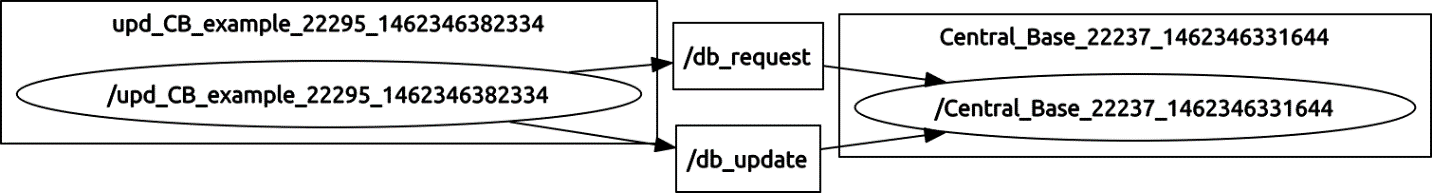
\includegraphics[width=0.4\textwidth]{TopicIntr1}
\caption{The initial communication with the central frame is made here. Each database, in its encrypted form, is created to be placed with each corresponding agent.}
\label{fig:TopicIntr1}
\end{figure}

A new connection is detected and notified via a list in topic /Host\_lists which signifies a working connection. Now, in order to test the appropriate data the testing node Simple\_calc.py was used as seen in Figure~\ref{fig:TopicIntr2}.

\begin{figure}[]
\centering
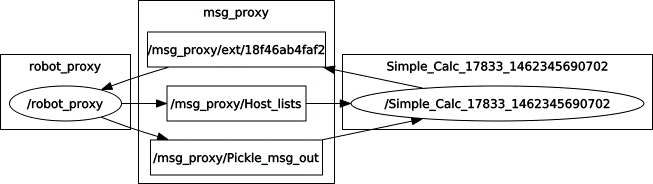
\includegraphics[width=0.4\textwidth]{TopicIntr2}
\caption{Topic Interaction with node- As new agents are populated, the external host lists are updated. Hence, when the topic handler retrieves the Host Lists from all the connection objects, the nodes in the current system will have an accurate overview of which topics are being published elsewhere based on the MAC of each external agent.}
\label{fig:TopicIntr2}
\end{figure}

Pickle\_msg out is the received messages from the outside world that are rebroadcasted. Each external agent connected has a subscriber created through /msg\_proxy/ext/. Scoping is utilized throughout to address each agent outside the current robot. The pickle\_msg contains a MAC field After setting up the correct interface to transfer frames over wifi things behaved like a regular wire. The OS was used in to set up a local network; with the secure nature of the messages exchanged this network can be left open so that future releases will not have difficulty communicating with older models. 

The results were, as expected, the node could not publish another type of message on our specified topic. Then, after making the appropriate PickleSend Type we are able to send the message to the subscriber callback in the robot proxy. From there we learn our transmission was successfully encrypted and transmitted through, received decrypted and unicasted to the receiving host. The process is carried on to the test bench of two zed boards where the implementation of response computation must be extendable to both the laptop and board despite architecture. We are able to verify the authentication and individual agent assignment by verifying the test data itself at each end of the connection.

\subsection{State Estimation}

\begin{table}[] \label{st_ctr_table}
\begin{center}
\begin{tabular}{|c|c|}
\hline
State & Control\\
\hline
$x,y,\theta,v_f,v_\theta$ & $a_f,a_\theta$\\
\hline
\end{tabular}
\end{center}
\end{table}

\subsection{Prediction}


\section{Results} \label{Results}
\subsection{Secure Ad-Hoc Channel Communication}



\subsection{State Estimation}



\subsection{Prediction}



\section{Conclusion} \label{Conclusion}
We have presented three components from a larger chain of trust that is designed to ensure security of not only the agent itself, but also of the group of agents surrounding it.

We have presented a simple distributed state estimation scheme operating over secure network channels that improves the performance of each agent and is augmented with a state detection scheme allowing agents to recognize possible subversive agents in their environment.
% conference papers do not normally have an appendix

% use section* for acknowledgment
\section*{Acknowledgment}
We would like to thank Professors Murat C. Cavusoglu, Russell C. Jackson and Tipakorn Greigarn and for their time, support and guidance.

\printbibliography
\end{document}
